\documentclass[preprint,12pt,number]{elsarticle}

\usepackage{amsmath,amssymb}
\usepackage{graphicx}
\usepackage{booktabs}
\usepackage{adjustbox}
\usepackage[section]{placeins}
% generated tables: small type, shrunk to the text width only if they are wider
\newcommand{\fittable}[1]{{\small\setlength{\tabcolsep}{4pt}\begin{adjustbox}{max width=\textwidth}\input{#1}\end{adjustbox}}}
\usepackage{siunitx}
\usepackage{xcolor}
\usepackage[hidelinks]{hyperref}

\sisetup{detect-all}
% Numbers that still wait for a run are marked like this, so nothing unchecked slips through.
\newcommand{\TBD}[1]{\textcolor{red}{[TBD: #1]}}
\newcommand{\Ub}{\bar U}
\newcommand{\bu}{\mathbf{u}}
\newcommand{\bv}{\mathbf{v}}
\newcommand{\bx}{\mathbf{x}}
\newcommand{\bw}{\mathbf{w}}
\newcommand{\dt}{\Delta t}

\journal{Computers \& Mathematics with Applications}

\begin{document}

\begin{frontmatter}

\title{Remeshing-induced force oscillations and computational cost in a GPU finite-element
projection solver}

\author[pdeu]{Anirudh Kulkarni}
\ead{anirudhk@outlook.in}
\affiliation[pdeu]{organization={School of Technology, Pandit Deendayal Energy University},
  city={Gandhinagar}, state={Gujarat}, country={India}}

\begin{abstract}
Dynamic mesh adaptation introduces velocity-transfer errors into projection methods and
additional work into GPU solvers. We quantify both for two-dimensional incompressible flow with
a P1--P1 finite-element solver (SUPG and orthogonal-subscale stabilisation), a BDF2 rotational
incremental projection scheme, and newest-vertex bisection with coarsening every 10\,ms. After
a remesh, both BDF2 velocity levels are transferred and re-projected with the scheme's
stabilised pressure operator, a projection-scheme form of the method of Braack, Lang and
Taschenberger (2013). In factorial ablations, an unstabilised projection targeting zero discrete
divergence produces drag second-difference excursions 300 to 400 times those of the
scheme-consistent re-projection at every remesh, whichever velocity levels are re-projected.
Retaining the stabilisation contribution in the rotational pressure update makes the pressure
error of a manufactured solution grow under time-step refinement. On the DFG 2D-2 and 2D-3
cylinder benchmarks the finest meshes reproduce the maximum drag to within 0.01\% and 0.03\%.
Adaptive refinement reduces the drag error per node at coarse resolution but not the wall time:
the finest adaptive run takes 736\,s against 259\,s for a uniform run of comparable drag
accuracy, because of remeshing overhead and twice as many momentum-solver iterations per step.
\end{abstract}

\begin{keyword}
Adaptive mesh refinement \sep newest-vertex bisection \sep GPU \sep projection method \sep
equal-order finite elements \sep flow past a cylinder \sep DFG benchmark
\MSC[2020] 65M60 \sep 65M50 \sep 65M12 \sep 76D05 \sep 65Y05
\end{keyword}

\end{frontmatter}

% =====================================================================================
\section{Introduction}
\label{sec:intro}

The laminar flow around a cylinder in a channel defined by \citet{schaefer1996} is the
standard test for incompressible solvers. Its periodic case (2D-2, Re = 100) and its
transient case (2D-3, inflow ramped up and down over $8\,$s) have reference values computed
with high-order finite elements on very fine meshes and small time steps
\citep{john2004,featflow}. Those values are known to four or five significant digits, so a
code can be checked against them far more tightly than against the original benchmark
intervals.

The flow is localised: a thin boundary layer, two separating shear layers and a vortex street
that moves downstream. Local refinement that follows these structures can reduce the number
of spatial degrees of freedom needed for a given accuracy, but its net computational benefit is
not obvious. It also adds
error sources that a fixed mesh does not have. Every remesh transfers the solution to a new
mesh; in a projection scheme the transferred velocity is no longer discretely divergence-free,
and the history levels that a multistep time integrator needs must be transferred as well.
On a GPU, where the solver itself is fast, the host-side remeshing can dominate the run time.
Adaptive finite-element results for the DFG benchmarks are usually goal-oriented and run on
CPUs \citep{braack2006,besier2012,bruchhaeuser2026}, and the effect of the remeshing itself on
the forces is rarely isolated. That a velocity moved to a new mesh is no longer discretely
divergence-free is well known, and the closest prior work addresses exactly this.
\citet{besierwollner2012} showed that interpolated or $L^2$-projected velocities perturb the
pressure on the new mesh by $O(1/\dt)$, distorting drag and lift, and proposed a discretely
divergence-free projection for inf--sup stable elements. \citet{braack2013} extended this to
stabilised equal-order elements: the transferred velocity is projected onto the
\emph{stabilised} divergence constraint, which contains the stabilisation term of the old
pressure; the multiplier of that projection enters the continuity equation of the following
time step; the projection is the identity on an unchanged mesh; and the pressure stays bounded
independently of $\dt$ for the Stokes equations with backward Euler. \citet{muller2019} transfer
all BDF history levels to the new mesh so that an adaptive BDF integrator keeps its order and
step size, and study grid-to-grid interpolation and the remeshing frequency for flow past a
square cylinder with monolithic Taylor--Hood elements. \citet{di2005} constructed a
divergence-preserving interpolation for moving-mesh finite elements, and
\citet{farrell2009,farrell2011} replaced nodal interpolation between unstructured meshes by
conservative Galerkin projection on a supermesh. In unfitted finite-element methods on moving
domains, the step-to-step change of the discrete problem causes spurious temporal oscillations
of the pressure; \citet{olshanskii2025} traced them to a loss of stability of the instantaneous
pressure and proposed a variant of the scheme that removes them. On the GPU side, finite-element
assembly on unstructured meshes \citep{cecka2011,markall2013} and adaptive finite-element
multigrid \citep{liebchen2024} have been studied, but the cost of frequent remeshing within a
time-dependent flow solver, measured against uniform refinement at equal accuracy, has received
less attention.

We ask two questions about a solver assembled from these standard components. How large are
the force errors that frequent remeshing introduces into a stabilised projection scheme, and
which parts of the transfer and of the time discretisation control them? And does adaptivity
reduce the wall time on a GPU at the accuracy of the reference data? The contribution is the
evidence for the answers, not a new formulation:
\begin{enumerate}
\item A pipeline for equal-order P1--P1 elements with SUPG and orthogonal-subscale (OSS)
  pressure stabilisation, BDF2 rotational incremental projection, and newest-vertex-bisection
  (NVB) refinement and coarsening at a fixed interval of 10\,ms, with assembly and solves on the GPU and
  the host remeshing overlapped with GPU time stepping (Section~\ref{sec:method}).
\item Five implementation choices that the verification showed to matter, three for the
  remeshing and two for the time discretisation, each measured by switching it off
  (Section~\ref{sec:ablation}). The re-projection after a remesh is the projection-scheme
  counterpart of the stabilised projection of \citet{braack2013}, applied to both BDF2 levels
  as \citet{muller2019} transfer their histories; we write out its equations, state where it
  differs from theirs, measure how far it is from the identity on an unchanged mesh, and
  separate by a factorial ablation the effect of the history level from that of the projection
  operator. For the rotational pressure term we derive what our variant omits.
\item A verification against the DFG reference data: a fully specified manufactured solution,
  spatial and temporal convergence on uniform and adaptive meshes, 2D-3, and the effect of
  the outlet condition, which differs from both references (Section~\ref{sec:verification}).
\item A cost account on one GPU that separates the gain per degree of freedom from the gain in
  wall time (Section~\ref{sec:cost}). The adaptive meshes are modestly ahead per node at the
  coarse end only, and not ahead in wall time. We give the breakdown that explains why.
\end{enumerate}

% =====================================================================================
\section{Problem and reference quantities}
\label{sec:problem}

The incompressible Navier--Stokes equations
\begin{equation}
\partial_t \bu + (\bu\cdot\nabla)\bu - \nu\Delta\bu + \nabla p = \mathbf{0},\qquad
\nabla\cdot\bu = 0
\label{eq:ns}
\end{equation}
are solved in the channel $\Omega = (0, 2.2)\times(0, 0.41)\,\mathrm{m}$ minus a cylinder of
diameter $D = 0.1\,$m centred at $(0.2, 0.2)$, with $\nu = 10^{-3}\,\mathrm{m^2/s}$;
$p$ is the kinematic pressure (pressure divided by the constant density), and all equations
below are written for it. The inflow is the parabola
$u(0,y) = 4U(t)\,y(H-y)/H^2$, $H = 0.41\,$m, and no-slip holds on the walls and the cylinder.

The two references treat the outlet differently. FEATFLOW, the 2D-2 reference, uses the
natural (do-nothing) outflow condition of its weak formulation \citep{featflow};
\citet{john2004}, the 2D-3 reference, prescribes the inflow parabola at the outlet as well.
Our default is the usual choice for a projection scheme: the pressure increment vanishes at
the outlet, and the momentum predictor has the natural condition
$\nu\,\partial_n\bu = \mathbf{0}$ there. Because the rotational update of
Section~\ref{sec:time-disc} acts at the outlet nodes too, the outlet pressure is not exactly
zero but carries the accumulated rotational correction; at $t = 8\,$s of 2D-2 it is below
$7\times10^{-4}$ in magnitude on U4 and below $0.016$ on A2 (the pressure difference across
the cylinder is about 2.5). Neither reference
condition is therefore matched exactly. Section~\ref{sec:outlet} repeats runs with the parabola
prescribed at the outlet and measures the effect.
\begin{itemize}
\item \textbf{2D-2:} $U = 1.5\,$m/s, mean velocity $\Ub = 1\,$m/s, Re $= \Ub D/\nu = 100$.
  The flow is run from rest to $t = 8\,$s; statistics are taken over the last full periods
  in $t \ge 6.5\,$s (Section~\ref{sec:2d2space} checks the remaining transient against runs to
  $t = 30\,$s). Reported are $C_{D,\max}$, $C_{D,\min}$, $C_{L,\max}$, $C_{L,\min}$, the
  Strouhal number St $= fD/\Ub$ from the lift period, and the pressure difference
  $\Delta p = p(0.15, 0.2) - p(0.25, 0.2)$ at half a period after the lift maximum, all with
  the definitions of the FEATFLOW reference data \citep{featflow}.
\item \textbf{2D-3:} $U(t) = 1.5\sin(\pi t/8)$ for $0 \le t \le 8\,$s, starting from rest.
  Reported are $C_{D,\max}$, $C_{L,\max}$, the times at which they occur, and
  $\Delta p(8\,\mathrm{s})$, against \citet{john2004}.
\end{itemize}
Drag and lift coefficients are $C_{D} = 2F_D/(\Ub^2 D)$ and $C_L = 2F_L/(\Ub^2 D)$, with
the forces per unit density and per unit depth and $\Ub = 1\,$m/s in both cases. The reference values are listed in
Tables~\ref{tab:2d2} and \ref{tab:2d3}.

% =====================================================================================
\section{Method}
\label{sec:method}

\subsection{Spatial discretisation}

Velocity and pressure are continuous piecewise-linear on triangles. Convection is written in
skew-symmetric form, $(\bw\cdot\nabla\bu, \bv) + \tfrac12((\nabla\cdot\bw)\bu, \bv)$, so the
Galerkin convection term does not inject energy when the discrete advecting velocity $\bw$ is
not exactly solenoidal \citep{skew}. Streamline-upwind Petrov--Galerkin (SUPG)
stabilisation \citep{brooks1982} adds the test function $\tau_K\,\bw\cdot\nabla\bv$ to the
mass, convection and pressure-gradient terms of the momentum predictor. The parameter is
\begin{equation}
\tau_K = \left[\left(\frac{2}{T}\right)^2 + \left(\frac{2|\bw|}{h_K}\right)^2
+ 9\left(\frac{4\nu}{h_K^2}\right)^2\right]^{-1/2},\qquad h_K = \sqrt{2|K|},
\label{eq:tau}
\end{equation}
in the transient form of \citet{tezduyar2000}. Usually $T = \dt$. We fix $T = 1\,$ms
instead, so that the spatial stabilisation does not change when $\dt$ is refined. With
$T = \dt$ the SUPG term perturbs the BDF2 time derivative by $O(\dt)$, and the observed
temporal order fell to one. The same inconsistency of a $\dt$-dependent $\tau$ was analysed by
\citet{jia2023}, who replace $\dt$ by a physical time scale computed every step from the ratio
of the $L^2$ norms of velocity and acceleration. Our constant $T$ is a fixed, flow-independent
approximation to such a time scale, and it is one more tuned constant;
Section~\ref{sec:ablation} measures the sensitivity to it. The transient term itself is needed: without it this
fractional-step scheme with a lagged pressure diverged on coarse cells (see \citet{bochev2004}
for the stability of transient SUPG). Section~\ref{sec:ablation} measures how much the results
depend on $T$.

Equal-order elements in a projection scheme need pressure stabilisation. We use orthogonal
subscales \citep{codina2000oss,codina2001}: the pressure Poisson operator is augmented by
\begin{equation}
S(q, r) = \sum_K s_K\,(\nabla q, \nabla r)_K
- \sum_i \frac{1}{m_i}\,G_i(q)\cdot G_i(r),
\label{eq:oss}
\end{equation}
where
\[
G_i(q) = \sum_{K\ni i}\sqrt{s_K}\,\frac{|K|}{3}\,\nabla q|_K,
\]
$s_K = \tau^p_K/\dt$, $\tau^p_K = c_{\rm oss}\,(4\nu/h_K^2 + 2|\bu^*|/h_K)^{-1}$,
and $m_i$ the lumped mass of node $i$. $S$ penalises only the part of $\sqrt{s}\,\nabla p$
that is orthogonal to its lumped $L^2$ projection onto continuous P1 functions, so smooth
pressures are not penalised. It is symmetric positive semi-definite. We treat the projection
implicitly, which keeps the operator SPD; a lagged projection over-damped the flow. The
factor $c_{\rm oss} = 0.3$ was set by the wall-pressure test of Section~\ref{sec:ablation}.
With $c_{\rm oss} = 0.03$ a node-to-node pressure mode appeared on the cylinder.

\subsection{Time discretisation}
\label{sec:time-disc}

The incremental pressure-correction scheme in rotational form \citep{timmermans1996,guermond2006}
is advanced with BDF2. With $\bw = 2\bu^n - \bu^{n-1}$ and $\dt' = 2\dt/3$, one step is:
\begin{enumerate}
\item momentum predictor for $\bu^*$ (both components with the same matrix):
\[
\frac{3\bu^* - 4\bu^n + \bu^{n-1}}{2\dt} + (\bw\cdot\nabla)\bu^* - \nu\Delta\bu^* + \nabla p^n = \mathbf{0},
\]
with SUPG and the Dirichlet data of time $t^{n+1}$;
\item pressure increment $\delta p$ from the stabilised Poisson problem
\[
(\nabla\delta p, \nabla q) + S(p^n + \delta p, q) = -\frac{1}{\dt'}(\nabla\cdot\bu^*, q);
\]
\item velocity correction $\bu^{n+1} = \bu^* - \dt'\,M_L^{-1}G\,\delta p$ with the lumped
  mass matrix $M_L$;
\item rotational pressure update $p^{n+1} = p^n + \delta p - \nu\,d^*$, where $d^*$ is a
  nodal approximation of $\nabla\cdot\bu^*$ discussed next.
\end{enumerate}
The first step is backward Euler.

\paragraph{The divergence in the rotational term}
Our $d^*$ is not the discrete divergence of $\bu^*$, and the difference matters. Let $K$ be the
P1 stiffness matrix, $S$ the matrix of \eqref{eq:oss}, and $D$ the discrete divergence,
$(D\bu)_i = (\nabla\cdot\bu, N_i)$. On every row without a pressure Dirichlet condition, step 2
reads $(K + S)\,\delta p = -(1/\dt')\,D\bu^* - S p^n$, so the lumped discrete divergence of
$\bu^*$ is exactly
\begin{equation}
M_L^{-1} D\bu^* = -\dt'\, M_L^{-1}\left[K\,\delta p + S\,(p^n + \delta p)\right].
\label{eq:divustar}
\end{equation}
In the continuous scheme $S = 0$ and $\nabla\cdot\bu^* = \dt'\,\Delta\delta p$. We use
the first term only,
\[
d^* = -\dt'\, M_L^{-1} K\,\delta p ,
\]
that is, the rotational correction is applied to the Galerkin part of the divergence and not to
the part that the stabilisation carries. Compared with $d^* = M_L^{-1} D\bu^*$, the update
therefore omits the term
\begin{equation}
\nu\,\dt'\,M_L^{-1} S\,(p^n + \delta p).
\label{eq:omitted}
\end{equation}
This is a modification of the scheme, not an identity. We have no stability proof for either
variant, and we keep the modification because of the observed behaviour, which the following
algebra helps to interpret. (i) The two variants differ only where $S(p^n+\delta p,\cdot)
\ne 0$, that is, only by the part of the pressure gradient that is orthogonal to its continuous
projection; for a pressure that $S$ does not penalise they coincide. (ii) If kept,
\eqref{eq:omitted} is added to the pressure explicitly at every step. $S$ is symmetric positive
semi-definite, so $M_L^{-1}S$ has non-negative eigenvalues, and taken in isolation the increment
amplifies the node-to-node modes that $S$ is meant to suppress; since $s_K = \tau^p_K/\dt$, the
factor $\nu\dt' s_K = \tfrac23\nu\tau^p_K$ does not depend on $\dt$, while the number of steps
grows like $1/\dt$. This is not a stability analysis: in the coupled scheme the pressure
increment, the stabilisation and the velocity correction interact. (iii) What we observe is
consistent with it. On U3 at $t = 0.1\,$s with $\dt = 1$, $0.5$ and $0.25\,$ms (fixed mesh, so
this is a pure time-step refinement), the $L^2$ pressure error of the manufactured solution with
our $d^*$ is $1.10$, $1.01$ and $0.97\times10^{-3}$, whereas with $d^* = M_L^{-1}D\bu^*$ it is
$0.97$, $2.84$ and $8.56\times10^{-2}$: it grows by about three each time $\dt$ is halved, and the
velocity error grows with it. Omitting \eqref{eq:omitted} prevents this growth in the present
discretisation. Section~\ref{sec:ablation} shows the effect on the benchmark.

\subsection{Forces}

Drag and lift are evaluated as volume integrals \citep{johnmatthies2001,john2004}:
\begin{equation}
F_D = -\left[(\partial_t\bu, \bv_d) + (\bu\cdot\nabla\bu, \bv_d) + \nu(\nabla\bu, \nabla\bv_d)
- (p, \nabla\cdot\bv_d)\right],
\end{equation}
with $\bv_d = (\chi, 0)$, where $\chi$ is the P1 function equal to one on the cylinder nodes
and zero elsewhere ($\bv_l = (0, \chi)$ for lift). The time derivative is the scheme's own
BDF2 difference. Only the layer of elements touching the cylinder contributes. Surface-traction
forces are computed as well, but only as a cross-check. $\Delta p$ is the difference of the
P1 pressure interpolated at the two probe points.

\subsection{Adaptive mesh}
\label{sec:amr}

\paragraph{Base mesh and bisection}
The base mesh has 508 nodes and 896 triangles: an O-grid in the square
$[0, 0.41]^2$ around the cylinder and a structured block downstream, with every quadrilateral
split along a diagonal. Both triangles of a quadrilateral get the diagonal as their refinement
edge. This satisfies Stevenson's matching condition, so newest-vertex bisection produces
conforming meshes with a bounded set of shapes, and the conformity closure only bisects
coarser elements \citep{mitchell1989,binev2004,stevenson2008}. One refinement level is two bisections
(it halves $h$). Midpoints of cylinder edges are projected onto the circle. Elements are kept
in a forest; coarsening removes newest vertices whose bisection patch is entirely marked for
coarsening, at most one level per adaptation. Every adapted mesh is checked (conformity,
orientation, boundary tags) before it is used. The minimum angle of the base mesh is
\ang{15.29}; no adapted mesh in this paper went below \ang{15.19}.

\paragraph{Indicators}
Both indicators measure the disturbance of the undisturbed channel flow. The inflow parabola
$u_P(y)$ has the same shear and curvature at every $x$; an indicator that sees it refines the
whole channel. We therefore subtract the nodal interpolant of $u_P$ (scaled with the current
inflow in 2D-3) from $u_h$ before recovering a continuous gradient $G'$ by area-weighted
averaging \citep{zienkiewicz1987,zienkiewicz1992}. On element $K$,
\begin{align}
\eta_{v,K} &= h_K \max_{i\in K}\left|\omega_i - \omega_P(y_i)\right|,\\
\eta_{i,K} &= \max_{\text{edges } e = (i,j)}\; \tfrac18\left|(G'_j - G'_i)\,\mathbf{e}\right|,
\end{align}
where $\omega$ is the recovered vorticity. $\eta_v$ is the velocity jump across the element
caused by rotation and shear. It sees the boundary layer, the shear layers and the shed
vortices. $\eta_i$ estimates the P1 interpolation error of the disturbance velocity. It sees
the stagnation and acceleration region in front of the cylinder, which carries little
vorticity but sets the surface pressure. In an early version of the code that used the
vorticity indicator alone, that region stayed coarse and $C_{L,\max}$ came out 8\% low.

\paragraph{Marking}
Each indicator is divided by its tolerance, $\hat\eta_v = \eta_v/\mathrm{tol}_v$ and
$\hat\eta_i = \eta_i/\mathrm{tol}_i$. Elements with $\max(\hat\eta_v, \hat\eta_i) > 1$ are
refined, largest first and within an element budget. Each element is refined by as many levels
as its worst indicator needs, using $\eta_v\sim h$ and $\eta_i\sim h^2$. An element is
coarsened only if its merged parent is predicted to stay below 0.35 on both indicators. The
band between 0.35 and 1 is a hysteresis that prevents refine--coarsen cycling. Four further
rules complete the marking:
\begin{itemize}
\item \emph{look-ahead}: indicators above tolerance are traced downstream with the local
  velocity over one adaptation interval and imposed along the path, so that shed vortices move
  into mesh that is already refined;
\item \emph{buffer and hole filling}: one layer of vertex neighbours is refined with each
  marked element, and an element coarser than two of its edge neighbours is refined;
\item \emph{minimum level}: no element is coarser than level 2. Because the indicators ignore
  the undisturbed parabola, the approach flow would otherwise stay on the base mesh;
\item \emph{keep radius}: no element whose centroid is within $0.25\,$m of the cylinder centre
  is coarsened.
\end{itemize}
In 2D-3 the tolerances are multiplied by $\max(|U(t)|/1.5, 0.1)$. With fixed tolerances the
mesh coarsened wholesale as the inflow died away, and remesh spikes contaminated
$\Delta p(8\,\mathrm{s})$.

The mesh is adapted every 10 steps ($10\,$ms at $\dt = 1\,$ms; the interval is scaled with
$\dt$ so that it stays $10\,$ms). Table~\ref{tab:levels} lists the three adaptive
configurations used throughout, and Fig.~\ref{fig:meshzoom} shows an A2 mesh.

\begin{figure}[!htbp]
\centering
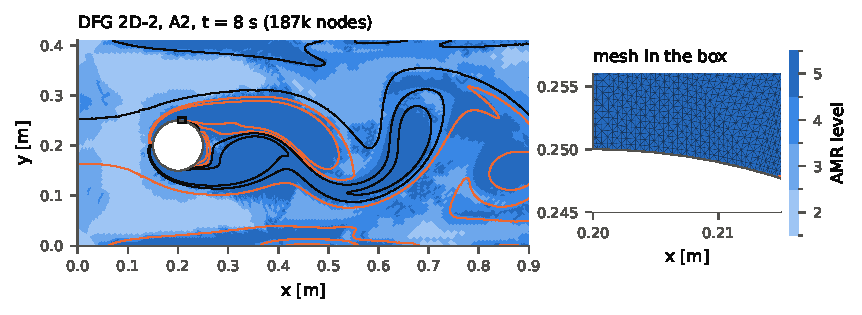
\includegraphics[width=\textwidth]{figures/fig_mesh_zoom.pdf}
\caption{DFG 2D-2, mesh A2 at $t = 8\,$s: refinement level with vorticity contours
($\omega = \pm5, \pm20\,\mathrm{s^{-1}}$), and the mesh in the small box on top of the cylinder.}
\label{fig:meshzoom}
\end{figure}

\begin{table}[!htbp]
\centering
\caption{Mesh configurations. Uniform meshes U$L$ refine the base mesh $L$ levels. Adaptive
meshes A1--A3 use the tolerances and maximum level shown, minimum level 2, adaptation every
$10\,$ms. Node counts are means over $t \ge 6.5\,$s of DFG 2D-2.}
\label{tab:levels}
\begin{tabular}{lrrrrr}
\toprule
mesh & tol$_v$ [m/s] & tol$_i$ [m/s] & max level & element budget & nodes (2D-2) \\
\midrule
U3 & -- & -- & 3 & -- & 29\,152 \\
U4 & -- & -- & 4 & -- & 115\,648 \\
U5 & -- & -- & 5 & -- & 460\,672 \\
A1 & 0.1   & 0.01   & 4 & 200\,000 & 50\,764 \\
A2 & 0.05  & 0.005  & 5 & 400\,000 & 187\,229 \\
A3 & 0.025 & 0.0025 & 6 & 1\,500\,000 & 707\,574 \\
\bottomrule
\end{tabular}
\end{table}

\paragraph{Transfer and re-projection}
On refinement, new midpoint values are interpolated linearly; on coarsening the values at the
remaining vertices are kept (injection). This transfer is neither conservative nor
divergence-preserving; conservative Galerkin projection on a supermesh \citep{farrell2009,
farrell2011} or a divergence-preserving interpolation \citep{di2005} are the principled
alternatives, and we did not try them. Both $\bu^n$ and $\bu^{n-1}$ are transferred, so the
BDF2 scheme keeps its history, as in \citet{muller2019}. The transferred fields do not satisfy
the discrete constraint of the scheme on the new mesh, and we re-project both levels with the
scheme's own pressure step. To make precise what this does, let $G$ be the discrete gradient,
$(Gq)_i = (\nabla q, N_i)$. In the implementation the velocity correction acts only on nodes
without a velocity Dirichlet condition (interior and outlet nodes), so $G$ and $M_L$ in the
correction are restricted to those nodes; $D$ acts on all nodal velocities, and the Dirichlet
values on the inlet, the walls and the cylinder enter it as data; the pressure equations are
taken on all rows except the outlet rows, where $\delta p = 0$. Midpoints created on the inlet,
the walls and the cylinder during refinement receive the exact Dirichlet values, so the transfer
preserves the boundary data. With these restricted operators, $E = K + DM_L^{-1}G$ is the
defect between the stiffness matrix and the Schur complement of the lumped projection. Steps 2 and 3 of a time step give, with
$p^n_* = p^n + \delta p$ the pressure before the rotational update,
\begin{equation}
D\bu^{n+1} + \dt'\,S\,p^n_* = -\dt'\,E\,\delta p ,
\label{eq:constraint}
\end{equation}
so $\bu^{n+1}$ satisfies the stabilised divergence constraint, not $D\bu = 0$, up to the
lumping defect. After a remesh, each transferred field $\tilde\bu$ is re-projected with the
current pressure $p$, which is not changed:
\begin{equation}
(K + S)\,\phi = -\frac{1}{\dt'}\,D\tilde\bu - S\,p,\qquad
\bu = \tilde\bu - \dt'\,M_L^{-1}G\,\phi,
\label{eq:reproj}
\end{equation}
hence
\begin{equation}
D\bu + \dt'\,S\,(p + \phi) = -\dt'\,E\,\phi .
\label{eq:reprojconstraint}
\end{equation}
This is the projection-scheme form of the stabilised projection of \citet{braack2013}, their
Eqs.~(12)--(13): with $q = \dt'\,\phi$ as the multiplier, the old-pressure term of their
constraint is our $\dt'\,Sp$ and their Darcy stabilisation $S^D_h$ is our $S$. It differs
from theirs in three respects. (i) It is an approximate projection: the mass matrix is lumped
and the Darcy Schur complement $-DM_L^{-1}G$ is replaced by $K$, which leaves the defect $E$.
(ii) It is applied to both BDF2 levels, each with the current pressure $p = p^n$. (iii) By
default the multiplier is discarded, whereas \citet{braack2013} add $-S^D_h(q_h,\cdot)$ to the
continuity equation of the next time step (their Eq.~(21)); the analogue here is to use
$S(p^n + \phi)$ instead of $Sp^n$ in the next pressure step. We have no counterpart of their
pressure bound.

Because of (i) and (ii) the re-projection is not exactly the identity on an unchanged mesh,
unlike their Lemmas~3 and 5. Inserting \eqref{eq:constraint} into \eqref{eq:reproj} for
$\tilde\bu = \bu^n$ on the same mesh gives
\[
(K + S)\,\phi = E\,\delta p - S\,(p^n - p^n_*),
\]
where $p^n - p^n_*$ is the rotational increment of step 4; in addition the weights $s_K$ are
re-evaluated with the current velocity. For $\bu^{n-1}$ the right-hand side also contains
$S$ applied to the pressure change over one step. All these terms are small, and
Section~\ref{sec:ablation} measures them by applying the re-projection every 10 steps on an
unchanged mesh.

The comparator in Section~\ref{sec:ablation}, which an earlier version of the code applied to
$\bu^n$ alone, is the unstabilised projection
\begin{equation}
K\,\phi = -\frac{1}{\dt}\,D\tilde\bu,\qquad
\bu = \tilde\bu - \dt\,M_L^{-1}G\,\phi,
\qquad\text{hence}\qquad
D\bu = -\dt\,E\,\phi ,
\label{eq:zeroproj}
\end{equation}
with the same restricted operators and the same pressure condition at the outlet. It targets
zero discrete divergence but, because the Schur complement is again replaced by $K$, reaches
it only up to the lumping defect; it is not an exact projection onto $D\bu = 0$. It is far from
the identity, because by \eqref{eq:constraint} it removes the stabilised part of the divergence
that the time step leaves. With it, the volume-integral drag shows a spike at every remesh
(Fig.~\ref{fig:remesh}).

\paragraph{Overlapped remeshing}
At a remesh step $n$ the indicators and the state are downloaded, and a host thread runs the
marking, refinement, coarsening, mesh extraction, CSR graph construction and validation. The
GPU meanwhile advances $K = 5$ more steps on the old mesh. At step $n + K$ the state of that
step is transferred to the new mesh with the same rules that the remesh would have used, and
the re-projection follows. The step at which the new mesh is used is fixed, so the results do
not depend on thread timing. The look-ahead horizon grows by $K$ steps. A unit test checks that
the transfer at $n + K$ reproduces the direct transfer bit for bit when the state has not
changed. In DFG 2D-2 the overlap changed the errors by at most 0.015 percentage points, and
in 2D-3 on A3 by at most 0.007 percentage points apart from $\Delta p(8\,\mathrm{s})$
(Sections~\ref{sec:ablation} and \ref{sec:limits}).

\subsection{GPU implementation and linear solvers}
\label{sec:gpu}

The code is written in CUDA C++ and uses double precision throughout. Element assembly uses
one thread per element with atomic additions into CSR matrices whose pattern is built once per
mesh. The momentum system (one matrix for both components) is solved by BiCGSTAB
\citep{vandervorst1992} with a multicolour ILU(0) preconditioner \citep{saad2003}, both
components in one solve, to a relative residual of $10^{-7}$. The pressure system is solved by
conjugate gradients with a smoothed-aggregation algebraic multigrid preconditioner
\citep{vanek1996} to a relative residual of $10^{-7}$. The OSS projection term of
\eqref{eq:oss} is applied inside CG as $-B^{\mathsf T}M_L^{-1}B$ with an assembled $B$. The AMG
setup (strength threshold 0.08, greedy aggregation, one damped Jacobi smoothing step of the
tentative prolongator, Galerkin coarse operators, dense inverse below 300 unknowns) runs on the
host with OpenMP after every remesh and at least every 50 steps; the symmetric V(2,2) cycle
with damped Jacobi smoothing runs on the GPU. The remeshing runs on the host (8 OpenMP threads).
The new mesh, the CSR pattern and the ILU colouring are then uploaded.

All runs in this paper used one NVIDIA RTX 5080 (16 GB) with an AMD Ryzen 9 9900X host,
CUDA 13.3 and gcc 13.3. Every timed run started only when no other process used the GPU, and
a watcher logged any other GPU process during the run. One ablation run overlapped another job
for about 30\,s; its errors are reported but its wall time is not.

% =====================================================================================
\section{Verification}
\label{sec:verification}

\subsection{Manufactured solution}

The manufactured solution is defined on the benchmark domain, with the cylinder, by a stream
function:
\begin{gather*}
\psi = \frac{A(t)}{b}\, f(x)\, g(y),\qquad u = \partial_y\psi,\qquad v = -\partial_x\psi,\\
p = \frac{A(t)}{2}\,\sin\big(k(L - x)\big)\cos(by),\qquad A(t) = 1 + \tfrac12\sin(10\pi t),\\
f(x) = \cos\big(k(x - L)\big) - \tfrac14\cos\big(2k(x - L)\big),\qquad g(y) = \sin(by) + \tfrac12\cos(by),\\
k = 2\pi/0.82\,\mathrm{m^{-1}},\qquad b = \pi/H,\qquad L = 2.2\,\mathrm{m}.
\end{gather*}
The velocity is exactly solenoidal. Since $f'(L) = f''(L) = 0$ and $p(L, y) = 0$, it satisfies
the outlet conditions of the code exactly ($\delta p = 0$ and $\nu\partial_n\bu = \mathbf{0}$),
and the outlet also fixes the pressure level, so no gauge correction is needed. The exact
velocity is prescribed at the inlet, the walls and the cylinder nodes. The body force
$\mathbf{f} = \partial_t\bu + (\bu\cdot\nabla)\bu - \nu\Delta\bu + \nabla p$
($\nu = 10^{-3}$) is evaluated at the nodes at $t^{n+1}$ and integrated as a P1 function with the
consistent mass matrix plus its SUPG weight. The run starts from the exact solution at $t = 0$.
The uniform meshes U1--U5 are run to $t = 0.1\,$s with $\dt\propto h$ ($\dt = 1\,$ms on U1),
so this is a coupled space--time refinement: the observed orders combine the spatial and temporal
errors.
Errors are absolute, measured at $t = 0.1\,$s on the polygonal computational domain with a
seven-point, degree-5 quadrature rule per triangle; $\max_\Gamma$ is the largest nodal pressure
error on the cylinder. Table~\ref{tab:mms} lists them. The velocity converges at the optimal
orders, two in $L^2$ and one in $H^1$. The pressure converges at between 1.5 and 2. Rotational
projection with $\dt \propto h$ predicts $O(\dt^{3/2})$ for the pressure \citep{guermond2006}.
The meshes in this test are fixed. Applying the remesh re-projection every 10 steps on these
fixed meshes leaves the errors unchanged to three significant digits
(Section~\ref{sec:ablation}), but the transfer between different meshes is verified only
through the benchmark convergence of the adaptive series and the ablations.

\begin{table}[!htbp]
\centering
\caption{Manufactured solution on uniform meshes, $\dt\propto h$, $t = 0.1\,$s.
Observed orders in brackets.}
\label{tab:mms}
\fittable{tables/tab_mms.tex}
\end{table}

\subsection{DFG 2D-2: spatial convergence}
\label{sec:2d2space}

All 2D-2 runs use $\dt = 1\,$ms and run to $t = 8\,$s.

\emph{Periodic state.} The FEATFLOW reference values are taken from a fully developed flow
(25--30\,s), whereas our statistics average the two lift periods in $6.5 \le t \le 8\,$s. The
flow is not yet exactly periodic there: on the finest meshes the two periods differ by
0.0024\% (U5) and 0.0025\% (A3) in $C_{L,\max}$, and by at most 0.001\% in $C_{D,\max}$, St and
$\Delta p$. To measure the remaining transient, U4 and A1 were run to $t = 30\,$s. On U4 the
statistics over $28.5 \le t \le 30\,$s differ from those over $6.5 \le t \le 8\,$s by 0.004
percentage points in $C_{L,\max}$ and $C_{L,\min}$ and by at most 0.0003 in $C_{D,\max}$, St and
$\Delta p$, and they no longer change after $t = 10\,$s. On A1 the differences are at most 0.003
percentage points. On these two meshes the 8-s statistics are therefore biased by up to about
0.004 percentage points in the lift. The other meshes were not run to $t = 30\,$s, so this is a
measured bias on U4 and A1 and the close agreement of the two periods on U5 and A3, not a
rigorous bound for every mesh; we quote it alongside the comparisons below.
 Table~\ref{tab:2d2} lists the errors
against FEATFLOW level 6, and Fig.~\ref{fig:eff} plots them against the mean number of nodes.
On the uniform meshes $C_{D,\max}$ and $C_{L,\max}$ converge at observed orders 1.98 and 2.14;
St converges at order 1.27. Richardson extrapolation of the uniform series gives
$C_{D,\max} = 3.22854$ and $C_{L,\max} = 0.98848$. The adaptive series gives orders 1.77 and
1.93 and extrapolates to $3.22787$ and $0.98883$. Both $C_{L,\max}$ extrapolations lie about
0.2\% above FEATFLOW. Section~\ref{sec:time} shows that this is the time error at
$\dt = 1\,$ms. $\Delta p$ does not converge monotonically on either series. It stays within
$+0.05\%$ to $+0.22\%$ of the reference; we return to it in Section~\ref{sec:limits}.

\begin{table}[!htbp]
\centering
\caption{DFG 2D-2, $\dt = 1\,$ms: relative error [\%] against FEATFLOW level 6
\citep{featflow}, mean nodes over $t\ge 6.5\,$s, and wall time of the whole run
($t = 0$--$8\,$s, one run each on an otherwise idle GPU).}
\label{tab:2d2}
\fittable{tables/tab_2d2.tex}
\end{table}


\begin{figure}[!htbp]
\centering
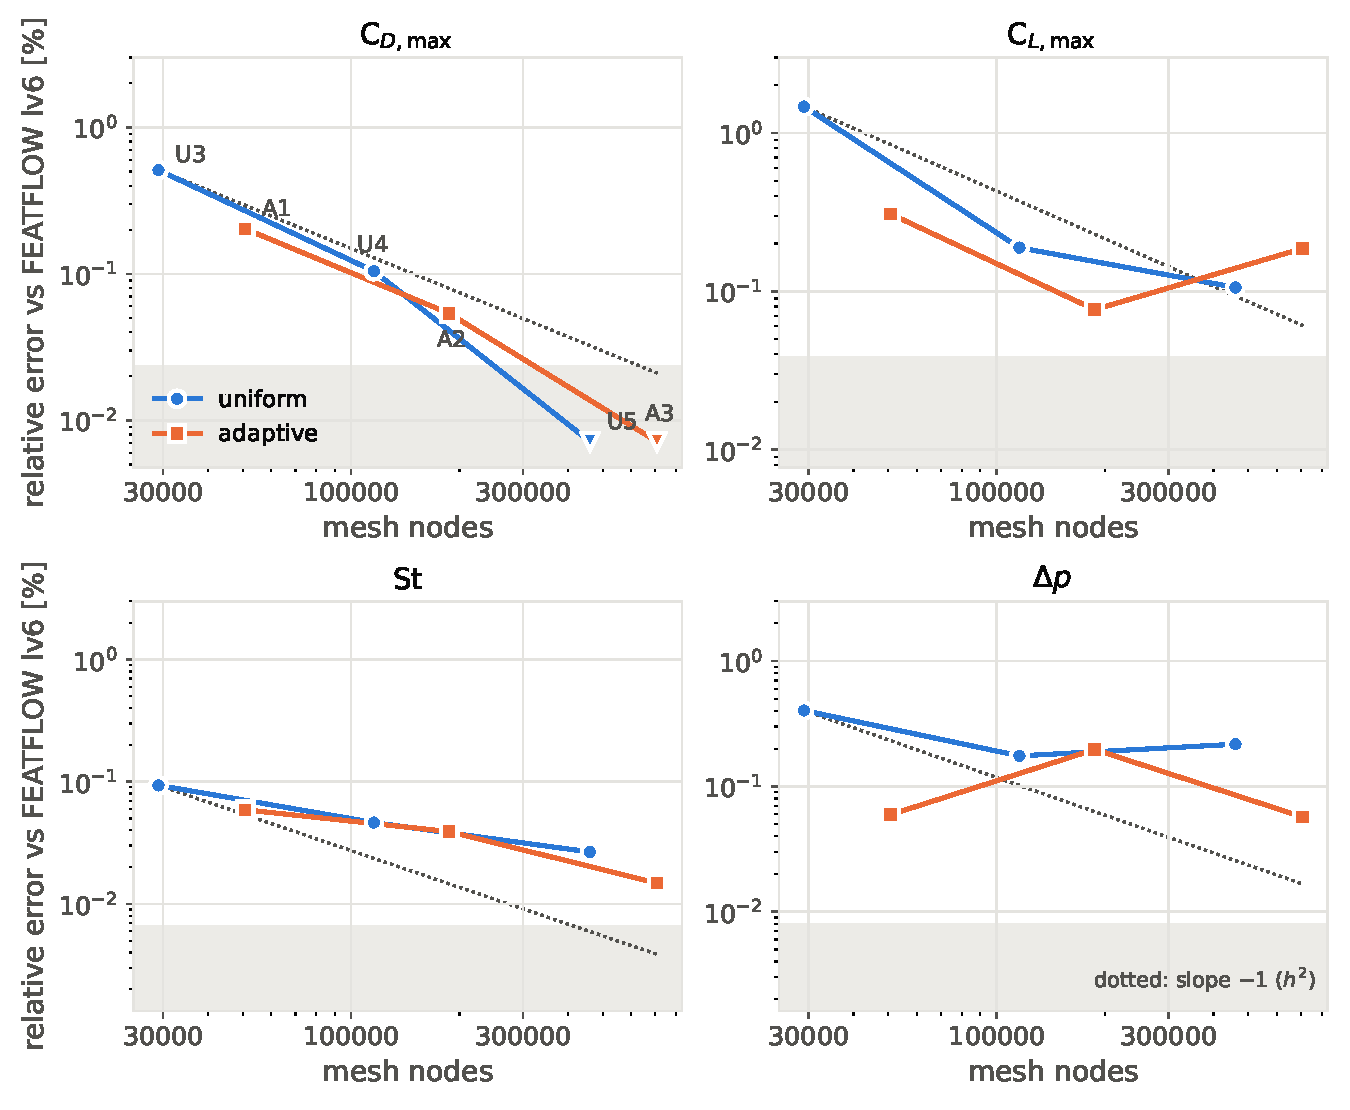
\includegraphics[width=0.8\textwidth]{figures/dfg2d2_efficiency_nodes.pdf}
\caption{DFG 2D-2, $\dt = 1\,$ms: absolute relative error against FEATFLOW level 6 versus
the mean number of nodes, for uniform (U3--U5) and adaptive (A1--A3) meshes. Dotted guide:
slope $-1$ (error $\propto h^2$). Grey band: difference between FEATFLOW levels 5 and 6.
Triangles mark errors below the plotted range. $C_{L,\max}$ includes the time error of about
$0.2\%$ at this time step (Section~\ref{sec:time}).}
\label{fig:eff}
\end{figure}

\begin{figure}[!htbp]
\centering
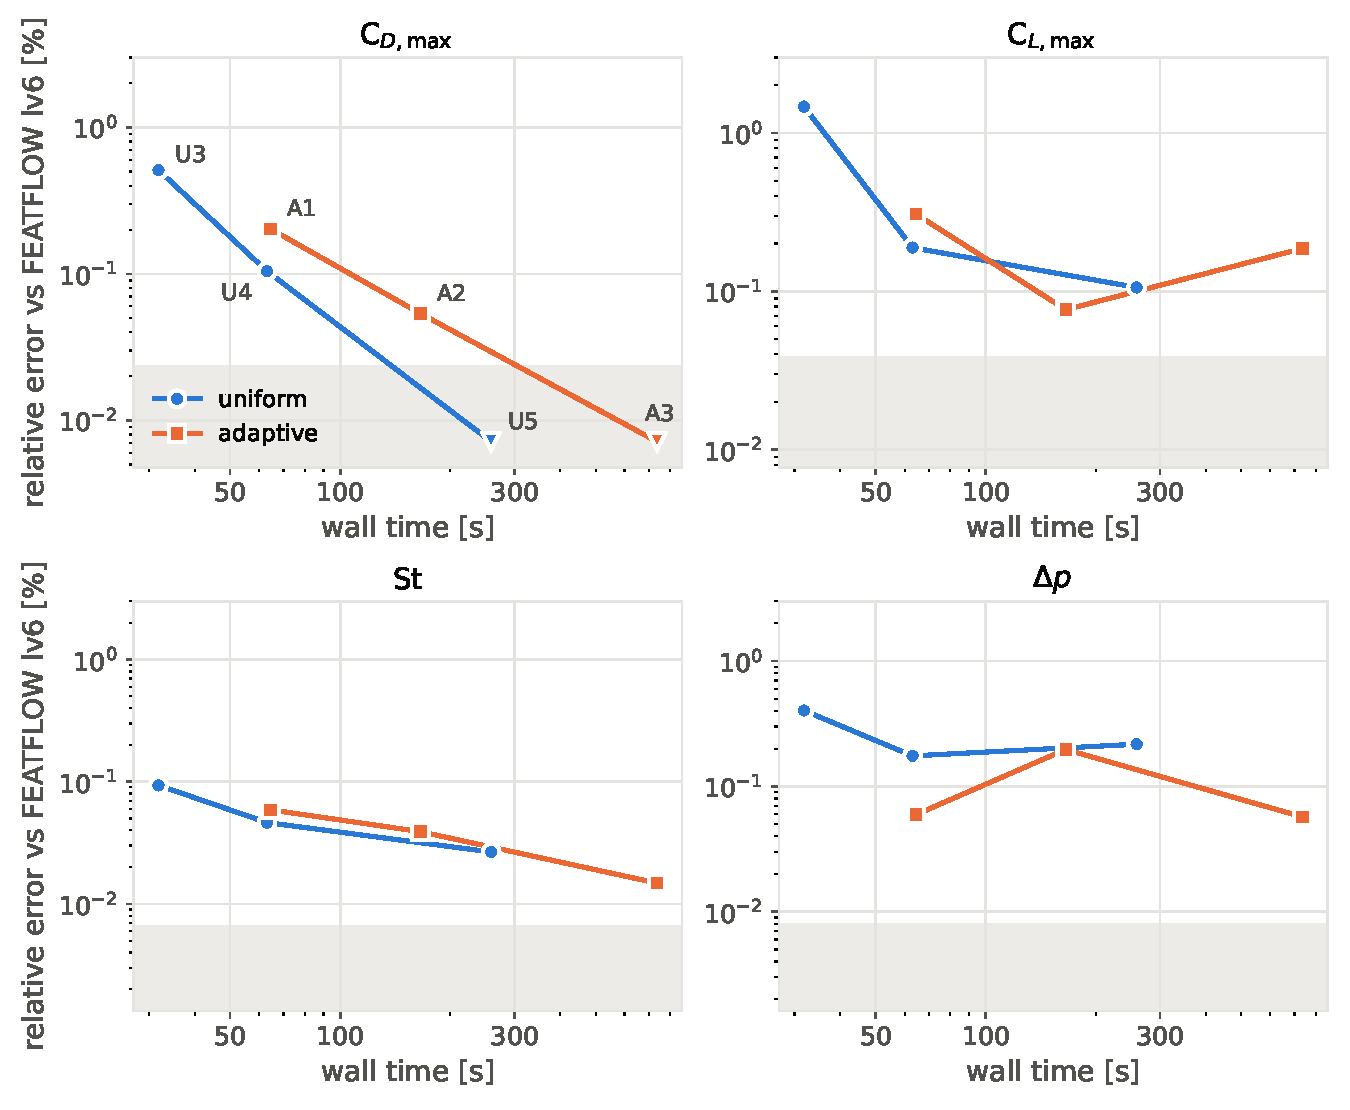
\includegraphics[width=0.8\textwidth]{figures/dfg2d2_efficiency_wall.pdf}
\caption{DFG 2D-2, $\dt = 1\,$ms: the errors of Fig.~\ref{fig:eff} versus the wall time of the
whole run ($t = 0$--$8\,$s, one run per mesh on an otherwise idle GPU).}
\label{fig:effwall}
\end{figure}

\subsection{DFG 2D-2: time step}
\label{sec:time}

On one adaptive and one uniform mesh, A2 and U4, $\dt$ was halved twice ($2$, $1$ and
$0.5\,$ms; on A2 the adaptation interval stays $10\,$ms). Table~\ref{tab:dt} shows
second-order convergence in time of the force maxima on both. On A2 the successive differences of $C_{D,\max}$ and
$C_{L,\max}$ fall by a factor of 4.16 (observed order 2.06), on U4 by 3.97 and 3.96.
Extrapolated at the observed order, the time error at $\dt = 1\,$ms is $+0.028\%$ in $C_{D,\max}$
and $+0.185\%$ in $C_{L,\max}$ on A2, and $+0.030\%$ and $+0.201\%$ on U4. The time error is thus
nearly the same on the two meshes, which differ in node count by 60\% and in mesh type; the two
estimates differ by 0.002 and 0.016 percentage points. $\Delta p$ does not show a clean order on
A2 (ratio 2.11, with changes below 0.04\%), although it does on U4 (4.07); we do not claim a
temporal order for it. This time error, not a spatial error,
is why the directly computed $C_{L,\max}$ of the finest meshes at $\dt = 1\,$ms is $+0.11\%$ (U5)
and $+0.19\%$ (A3) above FEATFLOW, and why both spatial extrapolations of $C_{L,\max}$ lie about
0.2\% above it.

The following space--time values are estimates, not computed results. They rest on the
assumption, supported by the two meshes above but not proven, that the time error at
$\dt = 1\,$ms is independent of the mesh. Subtracting from each spatial extrapolation the time
error measured on a mesh of the same family gives $C_{D,\max} = 3.22758$ and $C_{L,\max} =
0.98650$ for the uniform series ($+0.006\%$ and $-0.009\%$ against FEATFLOW level 6), and
$3.22698$ and $0.98700$ for the adaptive series ($-0.013\%$ and $+0.043\%$). Using the other
family's time error instead changes these estimates by at most 0.016 percentage points. For
comparison, FEATFLOW level 5 differs from level 6 by $-0.024\%$ and $-0.039\%$ in these two
quantities; this indicates the resolution of the reference data, not a rigorous error bound. The
estimates also carry the periodic-state bias measured on U4 and A1, up to 0.004 percentage points in the lift
(Section~\ref{sec:2d2space}); the outlet condition changes them by less than 0.001
(Section~\ref{sec:outlet}).

\begin{table}[!htbp]
\centering
\caption{DFG 2D-2, meshes A2 and U4: time-step study. Values and differences between
successive $\dt$.}
\label{tab:dt}
\fittable{tables/tab_dt.tex}
\end{table}

\subsection{DFG 2D-3}

Table~\ref{tab:2d3} compares the 2D-3 results with \citet{john2004}, and
Fig.~\ref{fig:d3history} shows the force histories. On A3, $C_{D,\max}$ is $-0.027\%$ from the
reference and its time is correct to $10^{-5}$ relative. $C_{L,\max}$ carries a time error at
$\dt = 1\,$ms. On U4 the values at $\dt = 1$, $0.5$ and $0.25\,$ms converge at second order in
time: the successive differences fall by a factor of 3.98, and the extrapolated value
0.47638 is $-0.33\%$ from the reference. On A2 the same refinement gives a ratio of 5.5, not a
clean order; its value at $\dt = 0.25\,$ms is $-0.28\%$ from the reference. At $\dt = 1\,$ms the
time error of about $+0.4\%$ therefore hides an offset of about $-0.3\%$ that is not a time
error, and it is not caused by the outlet condition either (Section~\ref{sec:outlet}). The A3
value at $1\,$ms is 0.19 percentage points above A2, so part of the offset is spatial; we did not run A3 at a smaller time step. $C_{D,\max}$ and the times of both maxima do
not depend on $\dt$ to within 0.015\%. $\Delta p(8\,\mathrm{s})$ is small ($-0.11$), flat in
$\dt$ on U4 ($-0.36$ to $-0.38\%$), and sensitive to the mesh history of the adaptive runs
(Section~\ref{sec:limits}).

\begin{table}[!htbp]
\centering
\caption{DFG 2D-3: relative error [\%] against \citet{john2004}; $t(\cdot)$ is the time of the
maximum. Meshes marked * prescribe the parabola at the outlet, as \citet{john2004} does
(Section~\ref{sec:outlet}); the others use our default outlet condition.}
\label{tab:2d3}
\fittable{tables/tab_2d3.tex}
\end{table}

\begin{figure}[!htbp]
\centering
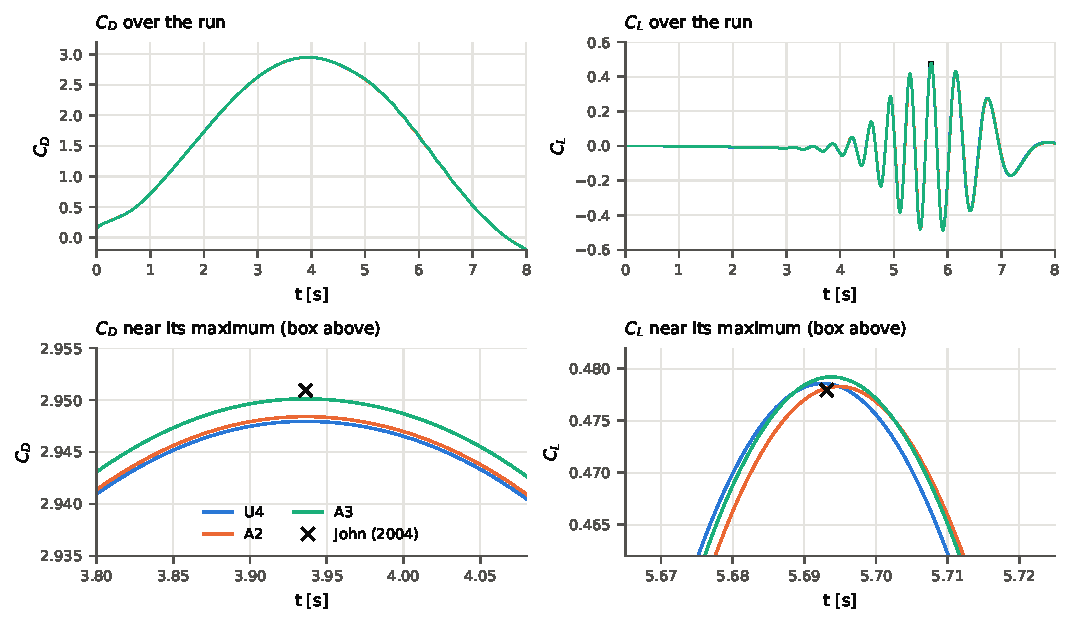
\includegraphics[width=\textwidth]{figures/fig_d3_history.pdf}
\caption{DFG 2D-3, $\dt = 1\,$ms: drag and lift histories on U4, A2 and A3 (top) and near the
maxima (bottom), with the reference maxima of \citet{john2004}.}
\label{fig:d3history}
\end{figure}

\begin{figure}[!htbp]
\centering
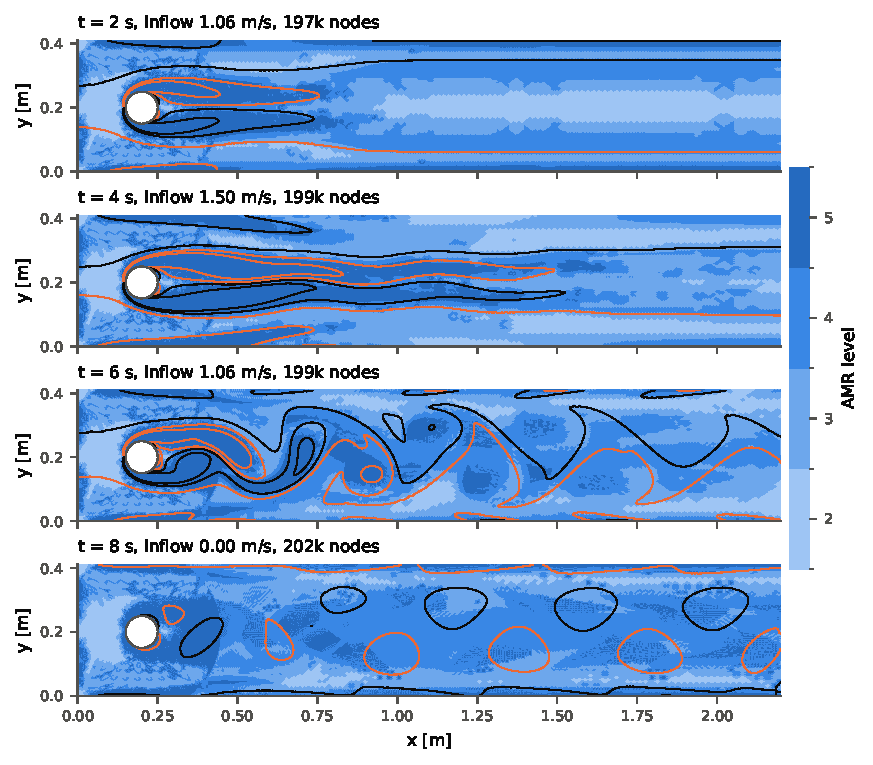
\includegraphics[width=\textwidth]{figures/fig_mesh_d3.pdf}
\caption{DFG 2D-3, mesh A2: refinement level and vorticity contours
($\omega = \pm5, \pm20\,\mathrm{s^{-1}}$) during the inflow cycle. The mesh follows the
growing wake and coarsens again as the inflow dies away.}
\label{fig:meshd3}
\end{figure}

\subsection{Outlet condition}
\label{sec:outlet}

To measure the effect of the outlet condition (Section~\ref{sec:problem}), we added the option
of prescribing the inflow parabola at the outlet, as \citet{john2004} does. The pressure is then
determined only up to a constant; the pressure increment is fixed at the outlet node nearest to
mid-height, after the right-hand side of the pressure equation has been made orthogonal to the
constants. On an adaptive mesh the inlet and outlet carry different nodes, and the trapezoidal
fluxes of the two interpolated parabolas then differ at $O(h^2)$, which makes the pressure
problem incompatible; we therefore scale the outlet parabola so that the two discrete fluxes
are equal. After a remesh the transferred outlet velocities of both time levels are rescaled
in the same way, so that the re-projection also sees a compatible flux; without this, every
coarsening of the outlet edges produced a one-step drag spike.

The effect on the forces is negligible (Tables~\ref{tab:outlet} and \ref{tab:2d3}). On U4 the
2D-2 quantities change by at most 0.0003 percentage points and the 2D-3 quantities, at all
three time steps, by at most 0.001; the time-extrapolated 2D-3 $C_{L,\max}$ is $-0.329\%$ from
\citet{john2004} with either condition, so its offset is not caused by the outlet condition.
On A1 the 2D-2 quantities change by at most 0.0004 percentage points. On the 2D-3 A2 mesh
$C_{D,\max}$ changes by 0.001 and $C_{L,\max}$ by 0.017 percentage points, and $\Delta p(8\,\mathrm{s})$
by 0.09, all within the mesh-history noise of adaptive runs (Section~\ref{sec:limits}). The
outlet lies 20 diameters downstream, and at Re $\le 100$ the forces do not see the difference
between the two conditions at the accuracy of this study. This also removes the outlet as the
suspected cause of the small $\Delta p$ offset in 2D-2.

\begin{table}[!htbp]
\centering
\caption{DFG 2D-2, $\dt = 1\,$ms: errors [\%] against FEATFLOW level 6 with our default outlet
condition ($p$) and with the parabola prescribed at the outlet.}
\label{tab:outlet}
\fittable{tables/tab_outlet.tex}
\end{table}

% =====================================================================================
\section{Diagnosis of remeshing-induced force oscillations}
\label{sec:ablation}

Section~\ref{sec:verification} established the accuracy of the complete solver. This section
asks which parts of it control the force errors, by switching one choice of
Section~\ref{sec:method} at a time on configuration A1 (DFG 2D-2, $\dt = 1\,$ms). Two
indicators are used. The force-oscillation indicator
\[
\mathcal{G} = \max_{n:\,t^n \ge 6.5\,\mathrm{s}} \left|C_D^{n+1} - 2C_D^n + C_D^{n-1}\right|
\]
is the largest temporal second difference of the drag, not a step-to-step change. On the fixed
mesh U3 it is $4.4\times10^{-5}$, the curvature of the smooth shedding signal at
$\dt = 1\,$ms. A global maximum does not by itself say where the excursion occurs, so for the
re-projection runs we also split it, using the node and element counts of the force history:
$\mathcal{G}_{\rm r}$ is the maximum over the steps whose second difference involves the first
step $m$ on a new mesh or the two steps after it ($m - 1 \le n \le m + 2$), and
$\mathcal{G}_{\rm o}$ the maximum over all other steps, so that
$\mathcal{G} = \max(\mathcal{G}_{\rm r}, \mathcal{G}_{\rm o})$. In every adaptive run of this section
$\mathcal{G} = \mathcal{G}_{\rm r}$. The
wall-pressure oscillation is the mean node-to-node oscillation of the pressure on the cylinder,
$|p_i - (p_{i-1} + p_{i+1})/2|$, at $t = 8\,$s.

\subsection{Re-projection after a remesh}

\begin{table}[!htbp]
\centering
\caption{Ablations on A1 (DFG 2D-2, $\dt = 1\,$ms): errors [\%] against FEATFLOW level 6,
force-oscillation indicator $\mathcal{G}$ and wall-pressure oscillation.}
\label{tab:ablation}
\fittable{tables/tab_ablation.tex}
\end{table}

Our re-projection differs from the simplest choice, the unstabilised projection
\eqref{eq:zeroproj} of $\bu^n$, in two ways: it treats both BDF2 levels, and it uses the
scheme's stabilised pressure step. Table~\ref{tab:reproj} switches the two independently. The
projection operator is what matters. With the unstabilised projection, $\mathcal{G}$ is
$2.9\times10^{-2}$ for $\bu^n$ alone and $2.3\times10^{-2}$ for both levels, 300 to 400 times
the $7.7\times10^{-5}$ of A1. The excursion is the same at every remesh: over the 150 remeshes
with $t \ge 6.5\,$s, the largest second difference near each remesh lies between $2.87$ and
$2.94\times10^{-2}$ ($\bu^n$ alone), and between $2.23$ and $2.28\times10^{-2}$ (both levels).
At the other steps the excursion has decayed but not vanished: $\mathcal{G}_{\rm o}$ is $9.4$ and
$8.2\times10^{-4}$, about 20 times the fixed-mesh value. With the scheme's
step, $\mathcal{G}_{\rm o}$ is $4.6\times10^{-5}$, the fixed-mesh value of U3, and the largest
second difference near a remesh is at most $7.7\times10^{-5}$ (median over the remeshes
$5.1\times10^{-5}$). The spikes of the unstabilised projection (Fig.~\ref{fig:remesh}) point
downwards and corrupt the extrema: $C_{D,\min}$ is
$-0.61\%$ or $-0.51\%$ instead of $-0.20\%$, and the apparently better $C_{D,\max}$ is an
artefact of the same spikes. With the scheme's step the spikes disappear whether one level or
both are re-projected; re-projecting $\bu^{n-1}$ as well halves the remaining $\mathcal{G}$
($1.4\times10^{-4}$ to $7.7\times10^{-5}$) and leaves the statistics unchanged to 0.003
percentage points. Not re-projecting at all is better than the unstabilised projection:
$\mathcal{G}$ is $6.1\times10^{-4}$, eight times that of A1 but 40 to 50 times smaller than with the
unstabilised projection, and the statistics move by at most 0.03 percentage points (St).
Adding the next-step term of \citet{braack2013} (last row) changes nothing measurable:
$\mathcal{G}$ is $7.5\times10^{-5}$ and the statistics move by at most 0.001 percentage points. The
history level and the projection operator thus have separable effects, and the operator
dominates: the time step leaves $\bu^n$ with the stabilised divergence of
\eqref{eq:constraint}, the unstabilised projection removes it, and the next pressure
step sees an artificial change of divergence at every remesh. An inconsistency between the two
BDF2 levels, the other plausible cause, is not the main one: making the levels consistent with the
unstabilised projection reduces $\mathcal{G}$ by only a fifth.

Table~\ref{tab:fixed} isolates the operator from the transfer: the same re-projections are
applied every 10 steps on the unchanged U3 mesh, so that an exact identity would change
nothing. With the scheme's step the velocity changes by at most $1.8\times10^{-5}$ per
re-projection (the velocity scale is 2), $\mathcal{G}$ rises from $4.4\times10^{-5}$ to
$9.0\times10^{-5}$, and the statistics change by at most 0.0003 percentage points; the next-step
term again makes no difference. The unstabilised projection changes the velocity by
$1.9\times10^{-3}$, a hundred times more, raises $\mathcal{G}$ 40- to 50-fold and moves the statistics
by up to 0.013 percentage points, on a mesh that does not change. The same test on the
manufactured solution (U1--U5, re-projection every 10 steps) leaves all errors of
Table~\ref{tab:mms} unchanged to three significant digits.

\begin{table}[!htbp]
\centering
\caption{Re-projection every 10 steps on the unchanged mesh U3 (DFG 2D-2, $\dt = 1\,$ms):
largest change of $\bu^n$ per re-projection (mean over $t \ge 6.5\,$s), $\mathcal{G}$, and
errors [\%] against FEATFLOW level 6. The first row is the plain U3 run.}
\label{tab:fixed}
\fittable{tables/tab_fixed.tex}
\end{table}

\begin{table}[!htbp]
\centering
\caption{Re-projection after a remesh on A1 (DFG 2D-2, $\dt = 1\,$ms): which velocity levels
are re-projected and with which operator (scheme step: \eqref{eq:reproj}; unstabilised:
\eqref{eq:zeroproj}). Errors [\%] against FEATFLOW level 6, and the force-oscillation indicator
near a remesh, $\mathcal{G}_{\rm r}$, and at all other steps, $\mathcal{G}_{\rm o}$ ($t \ge 6.5\,$s,
150 remeshes).}
\label{tab:reproj}
\fittable{tables/tab_reproj.tex}
\end{table}

\subsection{Mesh near the body, in the approach flow, and adaptation interval}

\emph{Keep radius.} If the elements near the cylinder may be coarsened, the mesh around the body
changes at every remesh. $\mathcal{G}$ grows 44 times, and $C_{L,\max}$ worsens from $-0.31\%$ to
$-0.94\%$.

\emph{Minimum level.} Without the floor the approach flow stays on the base mesh. The forces
then carry a bias that no refinement near the cylinder removes: $C_{D,\max}$ $-0.60\%$,
$C_{L,\max}$ $-0.87\%$ and St $-0.27\%$, about three times the drag and lift errors of A1 and four times its St error. The run costs
the same, so the minimum level improved the force accuracy without a measurable increase in wall
time.

\emph{Adaptation interval.} With the tolerances of A1 fixed and the mesh adapted every 5, 10
or 20\,ms (overlap $K$ = 2, 5 and 10 steps, look-ahead over one interval), $\mathcal{G}$ is
$7.8\times10^{-5}$, $7.7\times10^{-5}$ and $7.9\times10^{-5}$: the size of the remeshing
excursions does not depend on how often the mesh changes. The accuracy does, because the
refined region follows the shed vortices more closely when it is updated more often:
$C_{D,\max}$ is $-0.16\%$, $-0.20\%$ and $-0.22\%$ off and $C_{L,\max}$ $-0.23\%$, $-0.31\%$ and
$-0.35\%$, at nearly the same mean node count (51\,900, 50\,800 and 51\,700). The cost goes the
other way: the time spent in remeshing on the critical path is 35, 18 and 9\,s and the wall
time 80, 64 and 52\,s.

\subsection{Pressure stabilisation and the rotational term}

\emph{OSS factor.} With $c_{\rm oss} = 0.03$ the forces hardly change, but $\Delta p$ is
$+2.07\%$ off. The wall pressure carries a node-to-node mode eight times the oscillation of the
reference run (Fig.~\ref{fig:cp}).

\emph{Rotational term.} With $d^*$ taken as the full discrete divergence $M_L^{-1}D\bu^*$,
which retains the stabilisation contribution \eqref{eq:omitted}, the benchmark shows the same
wall-pressure mode as the small OSS factor, a $\Delta p$ error of $+0.57\%$, and twice the
$\mathcal{G}$ of A1. Together with the growth of the manufactured-solution pressure error under
time-step refinement (Section~\ref{sec:time-disc}), this is the evidence for omitting the
contribution in the present discretisation; the eigenvalue argument given there is an
interpretation, not a stability result for the coupled scheme.

\subsection{SUPG time scale and overlapped remeshing}

\emph{SUPG time scale.} Over $T = 0.5$--$2\,$ms every quantity changes by at most 0.04
percentage points.

\emph{Overlap.} Remeshing on the critical path instead of overlapping it changes the errors by
at most 0.015 percentage points and costs 7\% more wall time on A1. On A3 the overlap cut the
wall time from 963\,s to 736\,s.

\begin{figure}[!htbp]
\centering
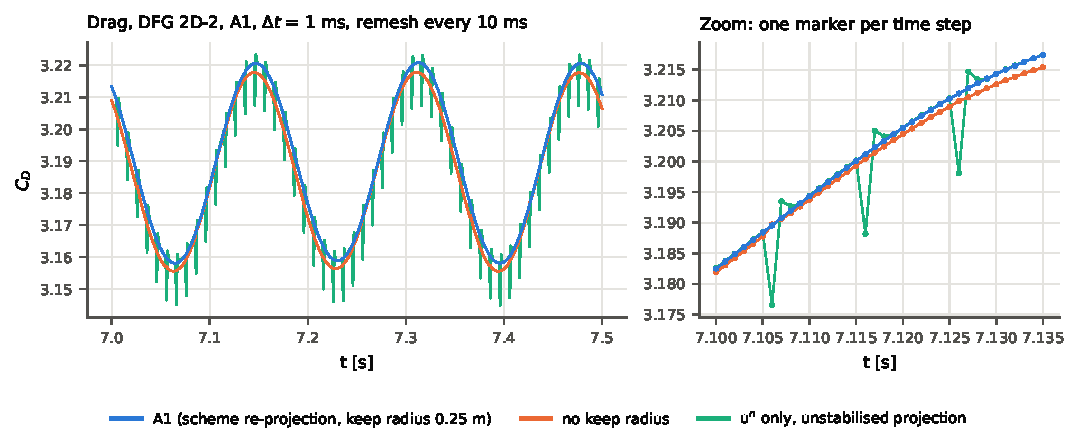
\includegraphics[width=\textwidth]{figures/fig_remesh.pdf}
\caption{DFG 2D-2, A1: drag with the scheme-consistent re-projection of both BDF2 levels and the
keep radius (A1), without the keep radius, and with the unstabilised projection \eqref{eq:zeroproj} of $\bu^n$ alone. The mesh is adapted every 10\,ms (10 steps).}
\label{fig:remesh}
\end{figure}

\begin{figure}[!htbp]
\centering
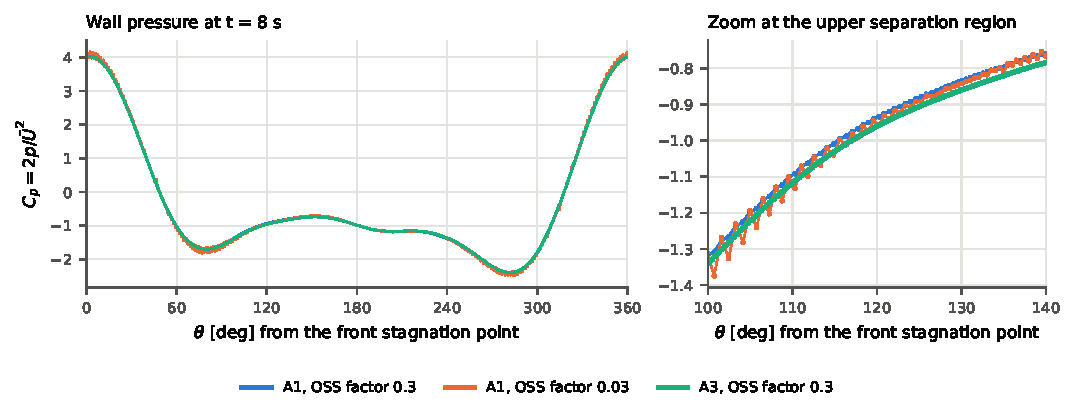
\includegraphics[width=\textwidth]{figures/fig_cp.pdf}
\caption{DFG 2D-2: pressure on the cylinder at $t = 8\,$s for A1 with OSS factor 0.3 and 0.03,
and for A3; $\theta$ is measured from the front stagnation point, through the upper side. The
pressure level is set by the outlet condition (Section~\ref{sec:problem}): the outlet pressure is
close to, but not exactly, zero.}
\label{fig:cp}
\end{figure}

% =====================================================================================
\section{Cost}
\label{sec:cost}

Fig.~\ref{fig:effwall} plots the errors of the runs of Table~\ref{tab:2d2} against
wall time. Per node, the adaptive meshes are ahead
only at the coarse end. Interpolating the uniform series at second order, A1 has about 1.5 times
smaller drag error than a uniform mesh with the same number of nodes and A2 about 1.2 times; A3
has more elements than U5 (1.41M against 0.92M) and no accuracy gain. In wall time the adaptive
meshes are not ahead. A1 and U4 take the same time (64 and 63\,s), and A1 has twice the drag
error ($-0.20\%$ against $-0.10\%$). A3 takes 736\,s for a $C_{D,\max}$ error of $-0.006\%$,
which U5 reaches in 259\,s, so A3 takes 2.8 times as long for the same drag error. Each wall time
is a single run; differences of a few per cent, such as 63 against 64\,s, are within the
run-to-run variation and are not interpreted.


Three effects contribute to the gap (Table~\ref{tab:cost}). First, the adaptive runs remesh 800
times. Even with the overlap, the exposed AMR work is 29\% of the A3 wall time: indicators,
upload, ILU colouring, the AMG setup for the new matrix and the re-projection solve. Second,
the solver costs more per node on adaptive meshes: BiCGSTAB needs 28 momentum iterations per
step on A3 against 14 on U5 (Table~\ref{tab:cost}). A3 has elements one level finer than U5
and transitions between refinement levels, and at a fixed $\dt$ the finer elements have larger Courant
numbers. We attribute the higher iteration count to this mesh-dependent conditioning of the
momentum system, but we have not isolated the Courant number, the grading or the element shape
experimentally. Third, the tolerances are uniform in space, so the far wake is resolved as
finely as the boundary layer. In the A3 mesh, 480k of the 1.4M elements are at the finest
level downstream of $x = 0.35\,$m, although the forces hardly depend on that region. A
distance-graded tolerance removed 40\% of the nodes in 2D-2 at little cost in accuracy, but
in 2D-3 it worsened $C_{L,\max}$ by 0.1 percentage points and brought back remesh-induced force excursions.
A goal-oriented indicator \citep{becker2001,fidkowski2011} is the principled fix, and we leave
it to future work.

\begin{table}[!htbp]
\centering
\caption{Wall-time breakdown of the DFG 2D-2 A3 and U5 runs [s].}
\label{tab:cost}
\fittable{tables/tab_cost.tex}
\end{table}

% =====================================================================================
\section{Limitations}
\label{sec:limits}

\begin{itemize}
\item \textbf{$\Delta p$ in 2D-2.} Our $\Delta p$ stays $+0.05$ to $+0.22\%$ above FEATFLOW
  and does not converge monotonically. The probe evaluation is not the cause: replacing the
  boundary-edge interpolation by local quadratic fits over 5--17 surface nodes changes $\Delta p$
  by 0.4\% on U3 and by 0.03\% on A3, a change that shrinks with refinement and changes sign
  between meshes. Nor is the outlet condition: prescribing the parabola there changes
  $\Delta p$ by less than $10^{-4}$ percentage points (Section~\ref{sec:outlet}), although we
  did not implement the do-nothing condition of FEATFLOW itself. The time error is $+0.02$ to
  $+0.03\%$ (Table~\ref{tab:dt}). The residual discrepancy remains unresolved.
\item \textbf{Mesh-history sensitivity.} Round-off-level changes, such as a different solver
  or the overlapped remesh, flip individual refine and coarsen decisions. The meshes then
  differ at about half the remesh steps, with node counts within 0.1\%. $C_D$ and $C_L$ change
  by less than $6\times10^{-5}$, but the 2D-3 $\Delta p(8\,\mathrm{s})$ on adaptive meshes
  moves by up to $\pm0.2\%$. We do not quote it more precisely than that. The overlapped
  remesh, which changes the mesh history more strongly, moved the 2D-3 $C_{L,\max}$ on A2 at
  $\dt = 1\,$ms from $+0.20\%$ to $+0.07\%$; on A3 it moved by only 0.007 percentage points.
  At $\dt = 1\,$ms this quantity carries a time error of about $+0.4\%$, so we read the A2 change
  as mesh-history noise on top of that error, not as a systematic effect.
\item \textbf{Wall time.} See Section~\ref{sec:cost}. The per-node advantage of the adaptive
  meshes does not translate into a wall-time advantage at the accuracy of the reference data
  on this hardware.
\item \textbf{Re-projection.} Our re-projection approximates the stabilised projection of
  \citet{braack2013} with a lumped mass matrix and the pressure-Poisson operator $K$ in place
  of the Schur complement. It is not exactly the identity on
  an unchanged mesh, and we have no stability bound for it; the evidence is the measurements of
  Section~\ref{sec:ablation}. The transfer itself is nodal interpolation and injection, neither
  conservative nor divergence-preserving.
\item \textbf{Scope.} Two-dimensional, laminar, one geometry. The indicators subtract the known
  inflow profile, which is specific to channel flows; for other flows the undisturbed state
  would have to be supplied or the plain recovered gradient used.
\end{itemize}

% =====================================================================================
\section{Conclusions}
\label{sec:conclusions}

\emph{Verification.} We verified a GPU P1--P1 finite-element projection solver with mesh
adaptation every 10\,ms on a manufactured solution and the DFG cylinder benchmarks. At
$\dt = 1\,$ms the finest meshes reproduce the 2D-2 maximum drag to within 0.01\% and the 2D-3
maximum drag to within 0.03\%. The 2D-2 maximum lift is 0.11--0.19\% high, which is its time
error at that step; this time error is nearly the same on a uniform and an adaptive mesh, and
removing it brings the extrapolated drag and lift within 0.05\% of the reference, an estimate
that assumes this mesh independence. The outlet condition changes the forces by less than
0.001 percentage points on uniform meshes, and stopping at $t = 8\,$s biases the lift
statistics by up to 0.004 percentage points on the two meshes run to $t = 30\,$s.

\emph{Diagnosis.} Five implementation choices were measured by ablation. The decisive one is to
re-project the transferred velocities with the scheme's own stabilised pressure step, a
projection-scheme form of the method of \citet{braack2013}. An unstabilised projection
targeting zero discrete divergence produced drag excursions at every one of the 150 remeshes
examined, with a second-difference indicator 300 to 400 times that of the scheme-consistent
re-projection, and was worse than no re-projection at all; with the scheme's step, the indicator
at steps away from a remesh equals the fixed-mesh value. The next-step term of
\citet{braack2013} made no measurable difference in our scheme, and on an unchanged mesh our
approximate re-projection is close to, but not exactly, the identity. The excursions do not
depend on the adaptation interval between 5 and 20\,ms. The other four choices are a
coarsening exclusion zone around the body, a minimum refinement level for the approach flow, an
SUPG time scale independent of $\dt$, and a rotational pressure update that omits the
stabilisation part of the discrete divergence; keeping that part made the manufactured-solution
pressure error grow as $\dt$ was refined.

\emph{Cost.} Per node, the adaptive meshes are 1.2 to 1.5 times more accurate than uniform ones
at the coarse end and not at the fine end. On one GPU they are not faster in wall time: the
finest adaptive run takes 2.8 times as long as a uniform run of the same drag accuracy, because
of remeshing, a higher solver cost per node and an indicator that is not goal-oriented. A
goal-oriented, adjoint-weighted indicator and a conservative or divergence-preserving transfer
are the next steps.


\section*{Code and data availability}
The solver source, the run scripts with every command line (mesh configurations of
Table~\ref{tab:levels}, adaptation parameters, solver tolerances), the force histories and
statistics of every run, and the scripts that regenerate every table and figure from them are
available at \url{https://github.com/rudhkul/cylinder-fem-amr} under the MIT licence. The VTK
solution fields (about 2\,GB) are not in the repository and are available from the author on
request.

\bibliographystyle{elsarticle-num-names}
\bibliography{refs}

\end{document}
